% A LaTeX template for MSc Thesis submissions to 
% Politecnico di Milano (PoliMi) - School of Industrial and Information Engineering
%
% S. Bonetti, A. Gruttadauria, G. Mescolini, A. Zingaro
% e-mail: template-tesi-ingind@polimi.it
%
% Last Revision: October 2021
%
% Copyright 2021 Politecnico di Milano, Italy. NC-BY

\documentclass{Configuration_Files/PoliMi3i_thesis}

%------------------------------------------------------------------------------
%	REQUIRED PACKAGES AND  CONFIGURATIONS
%------------------------------------------------------------------------------

% CONFIGURATIONS
\usepackage{parskip} % For paragraph layout
\usepackage{setspace} % For using single or double spacing
\usepackage{emptypage} % To insert empty pages
\usepackage{multicol} % To write in multiple columns (executive summary)
\setlength\columnsep{15pt} % Column separation in executive summary
\setlength\parindent{0pt} % Indentation
\raggedbottom  

% PACKAGES FOR TITLES
\usepackage{titlesec}
% \titlespacing{\section}{left spacing}{before spacing}{after spacing}
\titlespacing{\section}{0pt}{3.3ex}{2ex}
\titlespacing{\subsection}{0pt}{3.3ex}{1.65ex}
\titlespacing{\subsubsection}{0pt}{3.3ex}{1ex}
\usepackage{color}

% PACKAGES FOR LANGUAGE AND FONT
\usepackage[english]{babel} % The document is in English  
\usepackage[utf8]{inputenc} % UTF8 encoding
\usepackage[T1]{fontenc} % Font encoding
\usepackage[11pt]{moresize} % Big fonts

% PACKAGES FOR IMAGES
\usepackage{graphicx}
\usepackage{transparent} % Enables transparent images
\usepackage{eso-pic} % For the background picture on the title page
\usepackage{subfig} % Numbered and caption subfigures using \subfloat.
\usepackage{tikz} % A package for high-quality hand-made figures.
\usetikzlibrary{}
\graphicspath{{./Images/}} % Directory of the images
\usepackage{caption} % Coloured captions
%\usepackage[dvipsnames]{xcolor} % Coloured captions
\usepackage{xcolor} % Coloured captions
\usepackage{amsthm,thmtools,xcolor} % Coloured "Theorem"
%\usepackage{amsthm,thmtools} % Coloured "Theorem"
\usepackage{float}

% STANDARD MATH PACKAGES
\usepackage{amsmath}
\usepackage{amsthm}
\usepackage{amssymb}
\usepackage{amsfonts}
\usepackage{bm}
\usepackage[overload]{empheq} % For braced-style systems of equations.
\usepackage{fix-cm} % To override original LaTeX restrictions on sizes

% PACKAGES FOR TABLES
\usepackage{xltabular}
\usepackage{longtable} % Tables that can span several pages
\usepackage{colortbl}

% PACKAGES FOR ALGORITHMS (PSEUDO-CODE)
\usepackage{algorithm}
\usepackage{algorithmic}

% PACKAGES FOR REFERENCES & BIBLIOGRAPHY
\usepackage[colorlinks=true,linkcolor=black,anchorcolor=black,citecolor=black,filecolor=black,menucolor=black,runcolor=black,urlcolor=black]{hyperref} % Adds clickable links at references
\usepackage{cleveref}
\usepackage[square, numbers, sort&compress]{natbib} % Square brackets, citing references with numbers, citations sorted by appearance in the text and compressed
\bibliographystyle{abbrvnat} % You may use a different style adapted to your field

% OTHER PACKAGES
\usepackage{pdfpages} % To include a pdf file
\usepackage{afterpage}
\usepackage{lipsum} % DUMMY PACKAGE
\usepackage{fancyhdr} % For the headers
\fancyhf{}

% -----------
\usepackage{enumitem}
\usepackage{listings}
\usepackage{xltabular}

% Input of configuration file. Do not change config.tex file unless you really know what you are doing. 
% Define blue color typical of polimi
\definecolor{bluepoli}{cmyk}{0.4,0.1,0,0.4}

% Custom theorem environments
\declaretheoremstyle[
  headfont=\color{bluepoli}\normalfont\bfseries,
  bodyfont=\color{black}\normalfont\itshape,
]{colored}

% Set-up caption colors
\captionsetup[figure]{labelfont={color=bluepoli}} % Set colour of the captions
\captionsetup[table]{labelfont={color=bluepoli}} % Set colour of the captions
\captionsetup[algorithm]{labelfont={color=bluepoli}} % Set colour of the captions

\theoremstyle{colored}
\newtheorem{theorem}{Theorem}[chapter]
\newtheorem{proposition}{Proposition}[chapter]

% Enhances the features of the standard "table" and "tabular" environments.
\newcommand\T{\rule{0pt}{2.6ex}}
\newcommand\B{\rule[-1.2ex]{0pt}{0pt}}

% Pseudo-code algorithm descriptions.
\newcounter{algsubstate}
\renewcommand{\thealgsubstate}{\alph{algsubstate}}
\newenvironment{algsubstates}
  {\setcounter{algsubstate}{0}%
   \renewcommand{\STATE}{%
     \stepcounter{algsubstate}%
     \Statex {\small\thealgsubstate:}\space}}
  {}

% New font size
\newcommand\numfontsize{\@setfontsize\Huge{200}{60}}

% Title format: chapter
\titleformat{\chapter}[hang]{
\fontsize{50}{20}\selectfont\bfseries\filright}{\textcolor{bluepoli} \thechapter\hsp\hspace{2mm}\textcolor{bluepoli}{|   }\hsp}{0pt}{\huge\bfseries \textcolor{bluepoli}
}

% Title format: section
\titleformat{\section}
{\color{bluepoli}\normalfont\Large\bfseries}
{\color{bluepoli}\thesection.}{1em}{}

% Title format: subsection
\titleformat{\subsection}
{\color{bluepoli}\normalfont\large\bfseries}
{\color{bluepoli}\thesubsection.}{1em}{}

% Title format: subsubsection
\titleformat{\subsubsection}
{\color{bluepoli}\normalfont\large\bfseries}
{\color{bluepoli}\thesubsubsection.}{1em}{}

% Shortening for setting no horizontal-spacing
\newcommand{\hsp}{\hspace{0pt}}

\makeatletter
% Renewcommand: cleardoublepage including the background pic
\renewcommand*\cleardoublepage{%
  \clearpage\if@twoside\ifodd\c@page\else
  \null
  \AddToShipoutPicture*{\BackgroundPic}
  \thispagestyle{empty}%
  \newpage
  \if@twocolumn\hbox{}\newpage\fi\fi\fi}
\makeatother

%For correctly numbering algorithms
\numberwithin{algorithm}{chapter}

%----------------------------------------------------------------------------
%	NEW COMMANDS DEFINED
%----------------------------------------------------------------------------

% EXAMPLES OF NEW COMMANDS
\newcommand{\bea}{\begin{eqnarray}} % Shortcut for equation arrays
\newcommand{\eea}{\end{eqnarray}}
\newcommand{\e}[1]{\times 10^{#1}}  % Powers of 10 notation

%----------------------------------------------------------------------------
%	ADD YOUR PACKAGES (be careful of package interaction)
%----------------------------------------------------------------------------

%----------------------------------------------------------------------------
%	ADD YOUR DEFINITIONS AND COMMANDS (be careful of existing commands)
%----------------------------------------------------------------------------

%----------------------------------------------------------------------------
%	BEGIN OF YOUR DOCUMENT
%----------------------------------------------------------------------------

\begin{document}

\fancypagestyle{plain}{%
\fancyhf{} % Clear all header and footer fields
\fancyhead[RO,RE]{\thepage} %RO=right odd, RE=right even
\renewcommand{\headrulewidth}{0pt}
\renewcommand{\footrulewidth}{0pt}}

%----------------------------------------------------------------------------
%	TITLE PAGE
%----------------------------------------------------------------------------

\pagestyle{empty} % No page numbers
\frontmatter % Use roman page numbering style (i, ii, iii, iv...) for the preamble pages

\puttitle{
	title=ATD:\\Acceptance Testing Document,
	name1=Lorenzo Ferretti, % Author Name and Surname
	name2=Lorenzo Manoni, 
	name3=Carlo Sgaravatti,
	academicyear=2022-2023,
        version=1.0,
	date=05/02/2023,
        url=https://github.com/bighands2304/ManoniSgaravattiFerretti
} % These info will be put into your Title page 

%----------------------------------------------------------------------------
%	PREAMBLE PAGES: ABSTRACT (inglese e italiano), EXECUTIVE SUMMARY
%----------------------------------------------------------------------------
\startpreamble
\setcounter{page}{1} % Set page counter to 1

%----------------------------------------------------------------------------
%	LIST OF CONTENTS/FIGURES/TABLES/SYMBOLS
%----------------------------------------------------------------------------

% TABLE OF CONTENTS
\thispagestyle{empty}
\tableofcontents % Table of contents 
\thispagestyle{empty}
\cleardoublepage

%-------------------------------------------------------------------------
%	THESIS MAIN TEXT
%-------------------------------------------------------------------------
% In the main text of your thesis you can write the chapters in two different ways:
%
%(1) As presented in this template you can write:
%    \chapter{Title of the chapter}
%    *body of the chapter*
%
%(2) You can write your chapter in a separated .tex file and then include it in the main file with the following command:
%    \chapter{Title of the chapter}
%    \input{chapter_file.tex}
%
% Especially for long thesis, we recommend you the second option.

\addtocontents{toc}{\vspace{2em}} % Add a gap in the Contents, for aesthetics
\mainmatter % Begin numeric (1,2,3...) page numbering

\chapter{Tested Project}

\begin{itemize}
    \item\textbf{Authors}
        \begin{itemize}
            \item Andrea Bertogalli
            \item Nicolò Tombolini
            \item Niccolò Balestrieri
        \end{itemize}
    \item \textbf{GitHub repository:}
        \begin{itemize}
            \item https://github.com/andberto/BalestrieriBertogalliTombini
    \end{itemize}
    \item \textbf{Documents Considered:}
        \begin{itemize}
            \item RASD:\\https://github.com/andberto/BalestrieriBertogalliTombini/blob/main\\/DeliveryFolder/RASD3.pdf
            \item DD:\\https://github.com/andberto/BalestrieriBertogalliTombini/blob/main\\/DeliveryFolder/DD2.pdf
            \item ITD:\\https://github.com/andberto/BalestrieriBertogalliTombini/blob/main\\/DeliveryFolder/ITD1.pdf
    \end{itemize}
   
\end{itemize}

\chapter{Installation}

For the Installation setup, we have followed the instructions in the \emph{Installation Instructions} section of the ITD. The instructions to install the application server, the CPO app, and the end user app were very clear and detailed, and we didn't face any problems in making them run using the provided commands. However, we encountered some issues with the ChargingSocket application; indeed, the provided documentation didn't specify how to set up the connection with the server in order to test the QR-code scanning process and we had to request some further clarifications to make this work.

We already had MySQL and Node.js installed, so no further installations were needed in order to run the application server and the CPO application. In order to run the end-user application, the Flutter SDK was installed using the provided instructions.

Both the application server and the CPO application were run on a Windows 11 laptop. The CPO application was executed in Google Chrome. For the end-user application and the ChargingSocket application, we used some Android emulators from Android Studio; in particular:
\begin{itemize}
    \item The end-user application was tested in a Google Pixel 3A emulated on the Android Virtual Device (AVD) environment, with SDK version 33 and Android 13.0
    \item The ChargingSocket application was tested in a Google Pixel 4 emulated on the AVD environment, with SDK version 30 and Android 11.0
\end{itemize}

\chapter{Test cases}

\section{CPMS Test Scenarios}
\subsection{Register}
\begin{itemize}
    \item\textbf{Goals:}
        \begin{itemize}
            \item Register a new CPO.
        \end{itemize}
    \item \textbf{Steps:}
        \begin{itemize}
            \item Run the application 
            \item Push the 'Register Now' link
            \item Fill out all the fields required 
            \item Press the Sign-Up button. 
    \end{itemize}
    \item \textbf{Test Cases:}
        \begin{itemize}
            \item Providing all fields correctly
            \item Providing a password in the 'repeat password' field different from the first one
            \item Register with credential used yet.
    \end{itemize}
    \item\textbf{Test Result:}
        \begin{itemize}
            \item All cases were successfully executed.
    \end{itemize}
\end{itemize}

\subsection{Login}
\begin{itemize}
    \item\textbf{Goals:}
        \begin{itemize}
            \item Log in a CPO.
       \end{itemize}
    \item \textbf{Steps:}
        \begin{itemize}
            \item Run the application 
            \item Fill out all the fields required for the login. 
            \item Press the 'Login' button. 
        \end{itemize}
    \item \textbf{Test Cases:}
        \begin{itemize}
            \item Providing all fields correctly
            \item Providing an incorrect password
        \end{itemize}
    \item\textbf{Test Result:}
        \begin{itemize}
            \item If the credentials provided are correct, the system correctly logs the user into the application otherwise prevent the action.
        \end{itemize}
\end{itemize}

\subsection{Insert Charging Station}
\begin{itemize}
    \item\textbf{Goals}:
        \begin{itemize}
            \item Add a new Charging Station to the system. 
        \end{itemize}
    \item \textbf{Steps:}
        \begin{itemize}
            \item Login to the application.
            \item Navigate to the Charging Station page. 
            \item Press the 'Add a new station' button. 
            \item Fill out all required fields.
            \item Insert at least one socket  
            \item Press Confirm Button. 
        \end{itemize}
    \item \textbf{Test Cases:}
        \begin{itemize}
            \item Providing all fields correctly. 
            \item Providing all fields correctly without inserting any socket. 
        \end{itemize}
    \item\textbf{Test Result:}
        \begin{itemize}
            \item All cases were successfully executed. The CPO can't insert a new Charging Point without providing any socket. 
        \end{itemize}
\end{itemize}

\subsection{Update DSO Contract}
\begin{itemize}
    \item\textbf{Goals:}
        \begin{itemize}
            \item Change DSO provider for a certain Charging Station 
       \end{itemize}
    \item \textbf{Steps:}
        \begin{itemize}
            \item Login to the application.
            \item Navigate to the DSO Provider station page. 
            \item Press the 'Buy' button for a certain CP. 
            \item Press Confirm Button. 
        \end{itemize}
    \item \textbf{Test Cases:}
        \begin{itemize}
            \item Change DSO Provider. 
        \end{itemize}
    \item\textbf{Test Result:}
        \begin{itemize}
            \item The DSO provider is changed and the database system is updated.
        \end{itemize}
\end{itemize}

\subsection{Update Charging Mode}
\begin{itemize}
    \item\textbf{Goals:}
        \begin{itemize}
            \item Change the DSO-mode, DSO-mode, Auto-mode 
       \end{itemize}
    \item \textbf{Steps:}
        \begin{itemize}
            \item Login to the application.
            \item Navigate to the DSO Provider station page. 
            \item Choose between: Change the DSO-mode, Battery-mode, and Auto-mode with the toggle buttons
        \end{itemize}
    \item \textbf{Test Cases:}
        \begin{itemize}
            \item DSO-mode
            \item Battery-mode
            \item Auto-mode
        \end{itemize}
    \item\textbf{Test Result:}
        \begin{itemize}
            \item In all cases the information is updated in the DBMS. But there is no real implementation in the server in order to manage the automatic mode of both DSO and Battery cases. 
    \end{itemize}
\end{itemize}



\subsection{Monitor Charging Process}
\begin{itemize}
    \item\textbf{Goals:}
        \begin{itemize}
            \item Monitor the data relative to a Charging process happening. 
       \end{itemize}
    \item \textbf{Steps:}
        \begin{itemize}
            \item Login to the application.
            \item Navigate to the Battery Cluster status page
        \end{itemize}
    \item\textbf{Test Result:}
        \begin{itemize}
            \item The data displayed are correctly updated and reflect the behavior of the Charging Process. 
    \end{itemize}
\end{itemize}

\section {eMSP Test Scenarios}

\subsection{Login}
\begin{itemize}
    \item\textbf{Goals:}
        \begin{itemize}
            \item Login to the application
       \end{itemize}
    \item \textbf{Steps:}
        \begin{itemize}
            \item Run the Application. 
            \item Fill out all required fields. 
            \item Press the login button. 
        \end{itemize}
    \item \textbf{Test Cases:}
        \begin{itemize}
            \item Providing correct credentials
            \item Providing incorrect credentials 
        \end{itemize}
    \item\textbf{Test Result:}
        \begin{itemize}
            \item If the credentials are correct the system logs in the user correctly, otherwise an error message is displayed. 
        \end{itemize}
\end{itemize}

\subsection{Register}
\begin{itemize}
    \item\textbf{Goals:}
        \begin{itemize}
            \item Register in the application
       \end{itemize}
    \item \textbf{Steps:}
        \begin{itemize}
            \item Run the Application. 
            \item Insert the IP address of the server. 
            \item Fill out all the fields required for the registration
            \item Press the register button
        \end{itemize}
    \item \textbf{Test Cases:}
        \begin{itemize}
            \item Providing correct credentials
            \item Providing incorrect credentials 
            \item Providing correct IP address 
            \item Providing incorrect IP address 
        \end{itemize}
    \item\textbf{Test Results:}
        \begin{itemize}
            \item If the Ip-address provided is wrong the application doesn't allow the user to insert a new one and it can't access the application. 
            \item If the Ip-address provided is correct and the credentials are incorrect an error message is displayed.
             \item If the Ip-address and the credential are correct, the system registers the user successfully. 
        \end{itemize}
\end{itemize}

\subsection{Book a Charge}
\begin{itemize}
    \item\textbf{Goals:}
        \begin{itemize}
            \item Booking a Charging Session
       \end{itemize}
    \item \textbf{Steps:}
        \begin{itemize}
            \item Login to the application  
            \item Go to the Map View 
            \item Select a Charging Station
            \item Select a Time slot 
            \item Press the reserve Button.
        \end{itemize}
    \item \textbf{Test Cases:}
        \begin{itemize}
            \item Select a Time slot Free 
            \item Select a Time slot that is reserved. 
        \end{itemize}
    \item\textbf{Test Result:}
        \begin{itemize}
            \item If the time slot selected is reserved the reservation correctly fails and an error message is displayed. 
            \item If the time slot selected is free the reservation is correctly made. 
    \end{itemize}
\end{itemize}

\subsection{Delete a Booking}
\begin{itemize}
    \item\textbf{Goals:}
        \begin{itemize}
            \item Delete a Booking previously made. 
       \end{itemize}
    \item \textbf{Steps:}
        \begin{itemize}
            \item Login to the application  
            \item Press My Booking button. 
            \item Press on a Booking item.
            \item Press Delete Booking. 
        \end{itemize}
    \item\textbf{Test Result:}
        \begin{itemize}
            \item The booking is correctly eliminated from the system. 
    
    \end{itemize}
\end{itemize}

\subsection{Start Charging Process}
\begin{itemize}
    \item\textbf{Goals:}
        \begin{itemize}
            \item Start a charging Session. 
       \end{itemize}
    \item \textbf{Steps:}
        \begin{itemize}
            \item Login to the application  
            \item Navigate to 'My Bookings'
             \item Select a Booking  
            \item Scan the QR code on the socket via Charging Socket Application.
            \item Navigate to the Charge Status page. 
            \item Press 'Start Charging'. 
        \end{itemize}         
    \item \textbf{Test Cases:}
        \begin{itemize}
            \item Select a valid Booking (with a time range consistent, not expired...).  
            \item Select an invalid Booking (with a time range inconsistent)
        \end{itemize}
    \item\textbf{Test Result:}
        \begin{itemize}
            \item If the Booking is valid is possible to start the Charge, otherwise, the system prevents doing it.
    \end{itemize}
\end{itemize}


\subsection{Stop Charging Process}
\begin{itemize}
    \item\textbf{Goals:}
        \begin{itemize}
            \item Stop a Charging session started. 
       \end{itemize}
    \item \textbf{Steps:}
        \begin{itemize}
            \item Login to the application  
            \item Navigate to the Charge Status Page 
             \item Press the 'Stop Charging' button. 
        \end{itemize}         
    \item\textbf{Test Result:}
        \begin{itemize}
            \item The Charging is stopped correctly.
    \end{itemize}
\end{itemize}



\section{Additional points}
\subsection {Client applications}
\begin{itemize}
    \item There was a problem in the End User application with the WebSocket connection to the server in order to start a charging session after the QR-code scan. Indeed, with the provided configuration, the client wasn't able to establish a connection to the server due to a wrong endpoint. Figure~\ref{websocket} shows both the problem and the solution that we adopted to test the charging sessions.
    \begin{figure}[H]
        \centering
        \subfloat[\label{prob}]{
            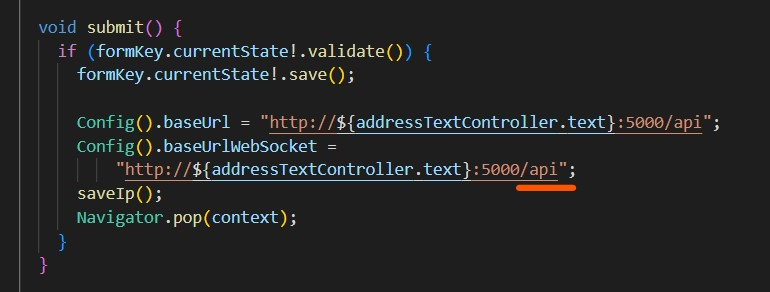
\includegraphics[scale=0.47]{Images/problem.jpg}
            }
        \quad
        \subfloat[\label{sol}]{
            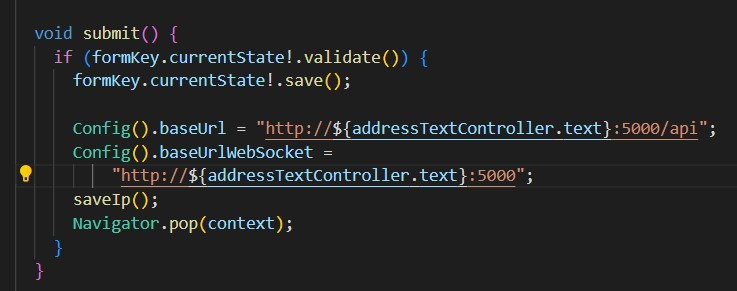
\includegraphics[scale=0.47]{Images/solution.jpg}
        }
        \caption{The WebSocket problem in the lib/view/set\_ip\_address.dart file (on the left), with the adopted solution (on the right).}
        \label{websocket}
    \end{figure}
    \item We appreciated the design of both the End User application and CPO application that allow easy and comfortable interaction with the system. 
\end{itemize}


\subsection {Application Server}
\begin{itemize}
       \item There is no access control for any operation provided to the server. For example, anyone can access data (e.g. from postman) and trigger any operation via API without any authentication.
        \item The code structure of the application server doesn't reflect the one provided in the component diagram of the DD. 
\end{itemize}

\subsection {RASD}
\begin{itemize}
       \item There is no management of any Optimizer (DSO energy acquisition and Battery Management). 
       \item The system can't interact with other systems since the communication standards are not respected. 
        \item  There is no control over the number of reservations that a user can make. Potentially a user can reserve all the sockets of all CPs in the application.
        \item A very good point in our opinion is the choice to insert a QR code verification to start a charging process since it prevents many possible issues that can happen in different otherwise.
\end{itemize}

\chapter{Effort Spent}

\section{Lorenzo Ferretti}

\begin{table}[H]
    \centering 
    \begin{tabular}{|l|c|c|}
    \hline
    \rowcolor{bluepoli!40}
    \textbf{Task} & \textbf{Hours Spent}\T\B \\
    \hline
    Testing & 8\T\B \\
    \hline
    \end{tabular}
\end{table}

\section{Lorenzo Manoni}

\begin{table}[H]
    \centering 
    \begin{tabular}{|l|c|c|}
    \hline
    \rowcolor{bluepoli!40}
    \textbf{Task} & \textbf{Hours Spent}\T\B \\
    \hline
    Testing & 8\T\B \\
    \hline
    \end{tabular}
\end{table}

\section{Carlo Sgaravatti}

\begin{table}[H]
    \centering 
    \begin{tabular}{|l|c|c|}
    \hline
    \rowcolor{bluepoli!40}
    \textbf{Task} & \textbf{Hours Spent}\T\B \\
    \hline
    Testing & 8\T\B \\
    \hline
    Environment installation & 2\T\B \\
    \hline
    \end{tabular}
\end{table}

\cleardoublepage

\end{document}
